%
% hilbertraum.tex
%
% (c) 2019 Prof Dr Andreas Müller, Hochschule Rapperswil
%
\section{Hilbertraum
\label{section:hilbertraum}}
\rhead{Hilbertraum}
Die bisher entwickelte Theorie ist aus zwei Gründen nicht ausreichend für das,
was wir vorhaben.

Ein endlichdimensionaler Vektorraum ist sicher ein geeigneter Rahmen zur
Beschreibung eines Signals, welches an endlich vielen Stellen abgetastet
wurde.
Für kontinuierliche Signale reicht er aber nicht.
Zunächst ist die Menge aller Funktionen zwar ein Vektorraum, aber es ist
aussichtslos, eine endliche orthonrmierte Basis zu finden.
Vielmehr werden wir sehen, dass bereits der Raum der stetigen Funktionen
auf einem Interval unendlich viele Funktionen enthält, die in einem noch
zu definierenden Sinn aufeinander senkrecht stehen.
Wir müssen daher den Begriff erweitern, so dass auch unendlichdimensionale
Vektorräume behandelt werden können.

In der Praxis tauchen nicht nur Signale mit rellen Werten auf, sondern
auch solche mit komplexen Werten.
An entscheidenden Stellen im vorangegangen Abschnitt, insbesondere bei
der Konstruktion der Norm, haben wir verwendet,
dass $0 \le x^2$ ist für $x\in\mathbb R$. Für $x\in\mathbb C$ ist dies
nicht mehr wahr.
Der bisher formulierte Begriff des Skalarproduktes funktioniert daher
nicht für komplexe Signale.

\subsection{Komplexe Vektorräume mit Skalarprodukt}
Es hindert uns nichts daran, in der Definition eines Vektorraums für die
Menge der Skalare auch komplexe Zahlen zuzulassen.
Ganz allgemein kann ein Vektorraum sinnvoll definiert werden, wenn die Menge
der Skalare ein sogenannter Körper ist, wenn also die Addition
und die Multiplikation mit von $0$ verschiedenen Skalaren umkehrbar sind.
Dies trifft natürlich für komplexe Zahlen zu, aber auch für $\mathbb Q$.

Die Definition der Länge eines Vektors und des Skalarproduktes auf dem
Vektorraum $\mathbb C^n$ erfordert aber etwas mehr Sorgfalt.
Die Quadratsumme der Komponenten funktioniert sicher nicht, da komplexe
Zahlen negative Quadrate haben können.
Die naheliegende Norm ist daher
\begin{equation}
\|v\| = \sum_{k=1}^n |v_k|^2.
\label{buch:hilbert:norm1}
\end{equation}
Sie ist für alle von $0$ verschiedenen Vektoren positiv, also positiv
definit.
Wir wollen diese Norm aber aus einem Skalarprodukt gewinnen.
Eine Möglichkeit ist
\begin{equation}
\langle u,v\rangle = \sum_{k=1}^n u_k\bar{v}_k.
\label{hilbert:skalaransatz}
\end{equation}
Die zugehörige Norm ist \eqref{buch:hilbert:norm1}.

Allerdings ist diese Bildung nicht mehr linear im zweiten Faktor.
Multipliziert man $v$ mit $\lambda$ erhält man
\[
\langle u,\lambda v\rangle
=
\sum_{k=1}^n u_k\bar{\lambda} \bar{v}_k
=
\bar{\lambda}\sum_{k=1}^n u_k\bar{v}_k
=
\bar{\lambda}\langle u,v\rangle.
\]
Man sagt, $\langle\;,\;\rangle$ ist {\em konjugiert linear} im zweiten Argument.
Im ersten Argument ist $\langle\;,\;\rangle$ aber immer noch linear.

Die Konstruktion~\eqref{hilbert:skalaransatz} ist auch nicht mehr
symmetrisch, vielmehr gilt:
\[
\langle v,u\rangle
=
\sum_{k=1}^n v_k\bar{u}_k
=
\overline{\sum_{k=1}^n u_k\bar{v}_k}
=
\overline{\langle u,v\rangle}.
\]
Vertauschen der Faktoren führt zum konjugiert komplexen Wert des
Skalarproduktes.
Man nennt diese Symmetrieeigenschaft von $\langle\;,\;\rangle$
{\em hermitesch}.
Hermitesche Formen zeichnen sich dadurch aus, dass
\[
\overline{\langle {\color{red}u},{\color{blue}u}\rangle}
=
\langle {\color{blue}u},{\color{red}u}\rangle.
\]
Nur die reellen Zahlen sind zu sich selbst konjugiert komplex, man kann
also schliessen, dass für eine hermitesche Form
$\langle u,u\rangle\in\mathbb R$ ist.

Dies führt uns auf die folgende Definition eines Skalarproduktes für einen
komplexen Vektorraum.
\begin{definition}
Eine Funktion
\[
\langle\;,\;\rangle
\colon V\times V\to \mathbb C : (u,v) \mapsto \langle u,v\rangle
\]
heisst ein komplexes Skalarprodukt, wenn gilt:
\begin{enumerate}
\item $\langle \;,\;\rangle$ ist linear im ersten Argument.
\item $\langle \;,\;\rangle$ ist konjugiert linear im zweiten Argument.
\item $\langle\;,\;\rangle$ ist hermitesch,
d.~h.~$\langle u,v\rangle=\overline{\langle v,u\rangle}$.
\item $\langle \;,\;\rangle$ ist positiv definit, d.~h.~es gilt
$\langle u,u\rangle \ge 0$ mit Gleichheit nur falls $u=0$.
\end{enumerate}
\end{definition}

Die Herleitung der Cauchy-Schwarz-Ungleichung hat die Symmetrie
und die Bilinearität des Skalarproduktes verwendet, sie lässt sich
also auf diese hermitesche Skalarprodukt nicht direkt übertragen.

\begin{satz}
Sei $V$ ein komplexer Vektorraum mit komplexem Skalarprodukt
$\langle\;,\;\rangle$,
dann gilt
\[
|\langle u,v\rangle| \le \|u\|\cdot \|v\|
\]
mit Gleichheit genau dann, wenn $u$ und $v$ linear abhängig sind.
\end{satz}

\begin{proof}[Beweis]
Wie im reellen Fall berechnen wird die Norm von $u+tv$:
\begin{align*}
0&\le
\| u+tv\|=\langle u+tv,u+tv\rangle
=
\|u\|^2 + \bar{t}\langle u,v\rangle + t\langle v,u\rangle + |t|^2 \|v\|^2
\\
&=
\|u\|^2 + \bar{t}\langle u,v\rangle + t\overline{\langle u,v\rangle} + |t|^2 \|v\|^2
\end{align*}
mit Gleichheit genau dann, wenn $u+tv=0$.
Die mittleren beiden Terme enthalten das Skalarprodukt, durch die Wahl
$t=-\langle u,v\rangle/\|v\|^2$ wird daraus
\begin{align*}
0
&\le
\|u\|^2 - 2\frac{|\langle u,v\rangle|^2}{\|v\|^2}
+
\biggl(\frac{|\langle u,v\rangle|}{\|v\|^2}\biggr)^2\|v\|^2
\\
&=
\|u\|^2 - \frac{|\langle u,v\rangle|^2}{\|v\|^2}.
\end{align*}
Multiplikation mit $\|v\|^2$ liefert
\begin{align*}
0&\le \|u\|^2 \cdot \|v\|^2 - |\langle u,v\rangle|^2
\\
\Leftrightarrow
\qquad
|\langle u,v\rangle|^2
&\le \|u\|^2 \cdot \|v\|^2
\end{align*}
mit Gleichheit genau dann, wenn $u+tv=0$.
Damit ist die Cauchy-Schwarz-Ungleichung auch für den komplexen Fall bewiesen.
\end{proof}

Auch für ein komplexes Skalarprodukt gilt, dass die Werte der Norm
das Skalarprodukt eindeutig bestimmen.
Da die Norm jedoch immer reelle Werte annimmt, ist etwas mehr Arbeit
erforderlich, um den Imaginärteil des Skalarproduktes wiederzugewinnen.
Znächst rechnen wir wie im Fall des reellen Skalarproduktes
\begin{align*}
\| u+v\|^2 
&=
\|u\|^2 + \langle u,v\rangle + \langle v,u\rangle + \|v\|^2
\\
&=
\|u\|^2 + \langle u,v\rangle + \overline{\langle u,v\rangle} + \|v\|^2
\\
&=
\|u\|^2 + 2\operatorname{Re}\langle u,v\rangle + \|v\|^2
\\
\Rightarrow\qquad
\operatorname{Re}\langle u,v\rangle
&=
\frac12(
\|u+v\|^2 - \|u\|^2 - \|v\|^2
).
\intertext{
Um den Imaginärteil zu bekommen, multiplizieren wir $v$ mit $i$:
}
\|u+iv\|^2
&=
\|u\|^2 + \langle u,iv\rangle + \langle iv,u\rangle + \|iv\|^2
\\
&=
\|u\|^2 -i \langle u,v\rangle + i\langle v,u\rangle + |i|^2 \|v\|^2
\\
&=
\|u\|^2 + \|v\|^2
-i (\langle u,v\rangle - \overline{\langle u,v\rangle})
\\
&=
\|u\|^2 + \|v\|^2
-i (2i\operatorname{Im}\langle u,v\rangle)
\\
&=
\|u\|^2 + \|v\|^2
+ 2\operatorname{Im}\langle u,v\rangle
\\
\Rightarrow\qquad
\operatorname{Im}\langle u,v\rangle
&=
\frac12(
\|u+iv\|^2- \|u\|^2 - \|v\|^2)
\end{align*}
Zusammengesetzt finden wir die Formel
\begin{equation}
\langle u,v\rangle
=
\frac12(
\|u+v\|^2 - \|u\|^2 - \|v\|^2
)
+
\frac{i}2(
\|u+iv\|^2- \|u\|^2 - \|v\|^2)
)
\label{hilbert:polarisierung}
\end{equation}
für das Skalarprodukt zweier beliebiger Vektoren, ausgedrückt
ausschliesslich mit der Norm.
Die Identität \eqref{hilbert:polarisierung} ist auch bekannt unter dem
Namen Polar-Identität oder Polarisierung des Skalarprodukts.
\index{Polar-Identität}
\index{Polarisierung}

Das Skalarprodukt erlaubt auch in einem komplexen Hilbertraum den Begriff
der orthonormierten Basis zu definieren.
\index{orthonormierte Basis}
Eine Menge von orthonormierten Vektoren ist automatisch linear unabhängig.
In einem $n$-dimensionalen Vektorraum reicht das um sicherzustellen,
dass eine Menge von $n$ orthonormierten Vektoren eine Basis ist.
In einem undendlichdimensionalen Vektorraum reicht Orthonormalität
jedoch nicht um sicherzustellen, dass sich jeder Vektor beliebig genau
als Linearkombination approximieren lässt.

\begin{definition}
Eine Menge von Vektoren $\mathcal{B} = \{v_1,v_2,\dots\}\subset H$ in einem
Hilbertraum $H$ heisst eine {\em Erzeugendensystem}, wenn es keinen Vektor
$v\in H$ gibt, der auf allen Vektoren von $\mathcal{B}$ senkrecht steht.
\end{definition}

\begin{beispiel}
Wir betrachten den Hilbertraum $l^2$, dessen Vektoren Folgen
$a=(a_k)_{k\in\mathbb N}$ von komplexen Zahlen sind mit dem Skalarprodukt
\begin{equation}
\langle a,b\rangle = \sum_{k\in\mathbb N} a_k\bar{b}_k.
\label{l2:beispiel:erzeugendensystem}
\end{equation}
Die Vektoren $e^{(i)}$ mit den Komponenten
\[
e^{(i)}_k = \delta_{ik}
\]
sind überall $0$ ausser das Folgenglied mit der Nummer $i$, welches $1$
ist. 
Diese Vektoren haben Länge $1$ im Sinne des Skalarproduktes
\eqref{l2:beispiel:erzeugendensystem} und sie sind orthogonal:
\[
\langle e^{(i)}, e^{(j)}\rangle
=
\sum_{k\in\mathbb N} e^{(i)}_k\bar{e}^{(j)}_k
=
\sum_{k\in\mathbb N} \delta_{ik}\delta_{jk}
=
\delta_{ij}.
\]
Die Vektoren $e^{(i)}$ sind aber auch ein Erzeugendensystem, wie man sich
wie folgt überzeugen kann.
Gäbe es einen Vektor $v\in l^2$, dessen Skalarprodukt mit allen $e^{(i)}$
verschwindet, dann würde für alle $i$ folgen
\[
0
=
\langle v,e^{(i)}\rangle
=
\sum_{k\in\mathbb N} v_ke^{(i)}_k
=
\sum_{k\in\mathbb N} v_k\delta_{ik}
=
v_i,
\]
d.~h.~der Vektor $v$ ist $0$.
\end{beispiel}

\begin{satz}
Wenn die Vektoren $\{e_k\,|\, 1\le k\le n\}$ eine orthonormierte Basis
von $V$ bilden, dann lässt sich jeder Vektor $v\in V$ als Linearkombination
\[
v
=
\sum_{k=1}^n \hat{v}_k e_k
\]
der Vektoren $e_k$ schreiben.
Die Koeffizienten sind eindeutig bestimmt und können mit Hilfe des
Skalarproduktes als
\[
\hat{v}_k = \langle v,e_k\rangle
\]
gefunden werden.
Ausserdem gilt für das Skalarprodukt die Plancherel-Identität
\index{Plancherel-Identität}
\begin{align*}
\langle u,v\rangle &= \sum_{k=1}^n \hat{u}_k\bar{\hat{v}}_k
\\
\| u \|^2 &= \sum_{k=1}^n |\hat{u}_k|^2.
\end{align*}
\end{satz}

Die Abbildung $T\colon V\to \mathbb C^n: v\mapsto (\hat{v}_k\,|\,1\le k\le n)$
ist also wie im reellen Fall eine {\em Isometrie}.
\index{Isometrie}


\subsection{Norm und Grenzwert in einem Hilbertraum}
Bis jetzt haben wir immer in endlichdimensionalen Vektorräumen gearbeitet.
Der tiefere Grund dafür war, dass die Arbeit mit unendlich vielen Basisvektoren
$e_k$, $k\in\mathbb N$, erfordert, dass Ausdrücken der Form
\begin{equation}
\sum_{k=1}^\infty a_k e_k
\label{hilbert:summe}
\end{equation}
einen Sinn gegeben werden muss.
Die Algebra reicht dazu nicht, denn zum Ende der Berechnung einer Summe
ohne Ende kann man grundsätzlich nicht gelangen.
Ein Ausdruck wie \eqref{hilbert:summe} kann daher nur im Sinne eines
Grenzwertes verstanden werden.
In einem Vektorraum ist aber a priori nicht definiert, wie man die
Approximation eines Vektors $v$ durch eine Folge von Vektoren $v_k$ zu
verstehen hat.

Mit der Einführung des Skalarproduktes und der daraus abgeleiteten Norm
ändert sich das.
\begin{definition}
Sei $V$ ein Vektorraum mit Skalarprodukt.
Eine Folge $v_k\in V$ konvergiert gegen den Vektor $v\in V$ für $k\to\infty$,
wenn
\[
\| v_k - v\| \to  0 
\qquad\Leftrightarrow\qquad
\lim_{k\to\infty} v_k = v.
\]
\end{definition}

Man erwartet, dass eine Folge einen Grenzwert hat, wenn die Folgenglieder
immer näher zu\-ei\-nan\-der rücken.

\begin{definition}
Eine Folge $v_k\in V$ heisst Cauchy-Folge, wenn es für jedes $\varepsilon > 0$
ein $N(\varepsilon)\in\mathbb N$ gibt, so dass
$\|v_k - v_m\| < \varepsilon$
sobald $k,m>N(\varepsilon)$.
\end{definition}

Leider ist nicht garantiert, dass in einem komplexen Vektorraum eine
Cauchy-Folge auch tatsächlich einen Grenzwert hat.

\begin{beispiel}
Wir betrachten den Vektorraum
\[
c_0 = \{ X=(x_0, x_1, \dots ,x_k,0,\dots)\,| x_i \in \mathbb C\}
\]
von Folgen, die nur endlich viele Terme haben, die von $0$ verschieden sind.
Wir können diesem Vektorraum ein Skalarprodukt verpassen, indem wir
\[
\langle X,Y\rangle
=
\sum_{k=1}^\infty x_k\bar{y}_k
\]
setzen.
Da in beiden Folgen nur endlich viele Terme von $0$ verschieden sind, ist
die Summe auf der rechten Seite eine endliche Summe.
Ganz offensichtlich ist dies ein komplexer Vektorraum mit Skalarprodukt.
Jetzt betrachten wir die Folge
\begin{align*}
X_1 &= (1,0,0,0,\dots)
\\
X_2 &= (1,\frac12,0,0,\dots)
\\
X_3 &= (1,\frac12,\frac13,0,\dots)
\\
&\vdots
\\
X_k &= (1,\frac12,\frac13,\dots,\frac1k,0,\dots)
\\
&\vdots
\end{align*}
Wir behaupten, dies sei ein Cauchy-Folge.
Dazu müssen wir Differentzen $\| X_n-X_m\|$ untersuchen.
Wir dürfen annehmen, dass $m < n$ ist.
Dann ist
\begin{equation}
\| X_n - X_m\|^2 = \sum_{k=m+1}^n \frac{1}{k^2}.
<
\sum_{k=m+1}^\infty \frac{1}{k^2}.
\label{hilbert:eulercauchy}
\end{equation}
Auf der rechten Seite steht ein Reststück der Reihe
\[
\sum_{k=1}^\infty \frac{1}{k^2},
\]
die Euler als erster berechnet hat.
Er hat den Wert $\frac{\pi^2}{6}$ gefunden.
Die Tatsache, dass die Reihe konvergiert heisst aber auch, dass
es für jedes $\varepsilon >0$ eine Zahl $N(\varepsilon)$ gibt derart,
dass die rechte Seite von \eqref{hilbert:eulercauchy} kleiner ist
als $\varepsilon$, wenn nur $m,n>N(\varepsilon)$.
Die Folge $(X_k)$ ist also tatsächlich ein Cauchy-Folge.

Als Grenzwert kommt nur die Folge 
\[
X = (1,\frac12, \frac13,\frac14,\dots)
\]
in Frage.
Und tatsächlich ist
\begin{equation}
\|X-X_n\|^2
=
\sum_{k=n+1}^\infty \frac1{k^2},
\label{hilbert:falscherabstand}
\end{equation}
wieder ein Reststück der Reihe von Euler.
Also konvergiert tatsächlich $X_k$ gegen $X$.

Die Folge $X$ ist aber gar nicht in $c_0$,
da alle Folgenglieder von $0$ verschieden sind.
Der Grenzwert einer Folge in $c_0$ muss also nicht mehr in $c_0$ sein.

Genau genommen haben wir schon in \eqref{hilbert:falscherabstand}
gemogelt.
Die Abstandsmessung in $c_0$ ist ja mit Hilfe einer endlichen Summe
definiert, hier haben wir aber eine unendliche Summe.
\end{beispiel}

Die Rekonstruktion eines Vektors mit Hilfe einer Linearkombination von
Basisvektoren kann also grundsätzlich nur dann funktionieren, wenn verlangt
wird, dass es zu jeder Cauchy-Folge von Vektoren auch tatsächlich einen
Grenzwert gibt.

\begin{definition}
Ein komplexer Vektorraum $V$ mit Skalarprodukt heisst {\em vollständig}, 
wenn jede Cauchy-Folge von Vektoren in $V$ einen Grenzwert in $V$ hat.
Ein solcher Vektorraum heisst {\em Hilbertraum}.
\end{definition}

Der Vektorraum $c_0$ des obigen Beispiels lässt sich leicht zu einem
Hilbertraum machen.

\begin{beispiel}
Sei $l^2$ der komplexe Vektorraum der quadratsummierbaren komplexen
Zahlfolgen $(x_k)$, d.~h.
\[
l^2 = \left\{ (x_k)\,\left| \sum_{k=1}^\infty |x_k|^2 < \infty \right.\right\}
\]
mit dem Skalarprodukt
\[
\langle X,Y\rangle = \sum_{k=1}^\infty x_k\bar{y}_k.
\]
% XXX TODO: Vervollständigung: Summierbarkeit des Grenzwertes...
\end{beispiel}

\subsection{Basis eines Hilbertraumes}

\begin{beispiel}
\label{geometrie:l2-beispiel}
\begin{figure}
\centering
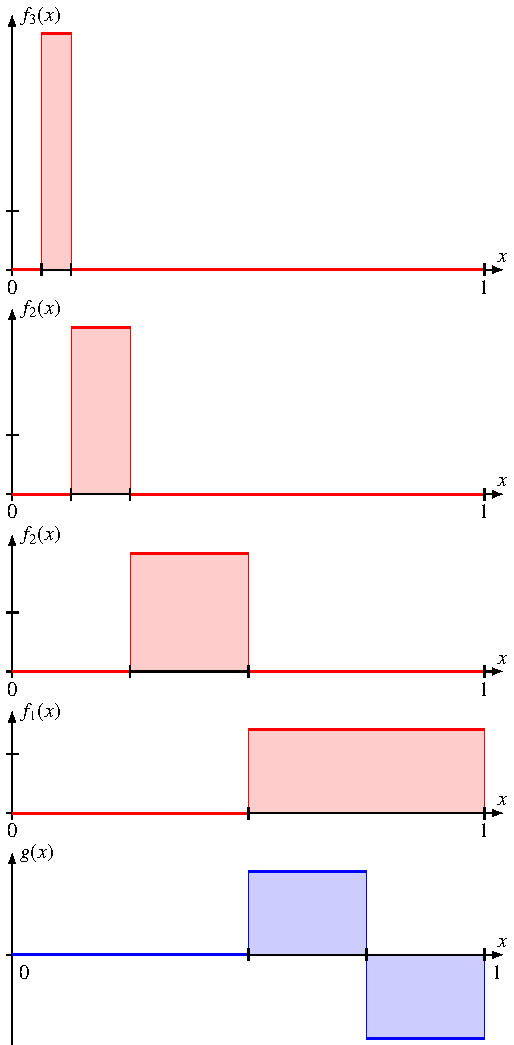
\includegraphics{chapters/1-geometrie/images/l2orth.pdf}
\caption{Familie von orthnormierten Funktionen $f_n(x)$, die alle auf der
Funktion $g(x)$ orthogonal sind.
Es gilt also $\langle f_n,f_m\rangle = \delta_{nm}$ und
$\langle f_n,g\rangle=0$.
\label{l2orth}}
\end{figure}
Wir zeigen Anhang eines Beispiels, dass der Vektorraum  der integrierbaren
Funktionen auf dem Interval $[0,1]$ mit einem Skalarprodukt
ausgestattet werden kann, welches ihn zu einem Hilbertraum macht.
Ausserdem konstruieren wir eine unendliche Menge von Funktionen, die alle
senkrecht aufeinander stehen.
Trotzdem werden wir einen weiteren Vektor finden, der auf all diesen
Vektoren senkrecht steht.

Als erstes definieren wir das Skalarprodukt von Funktionen auf dem
Interval $[0,1]$ als
\[
\langle f, g\rangle
=
\int_0^1 f(x) \bar{g}(x)\,dx
\]
für Funktionen $f,g\colon [0,1]\to\mathbb C$.
Der Vektorraum der integrierbaren Funktionen mit diesem Skalarprodukt
heisst $L^2$ und wird in Kapitel~\ref{chapter:fourier} genauer untersucht.

Als nächstes konstruieren wir die Folge $f_i$ von Funktionen, die wie
folgt definiert sind:
\begin{align*}
f_1(x) &= \begin{cases}
\sqrt{2}&\qquad \frac12x1\\
0\phantom{000}&\qquad\text{sonst}
\end{cases}
\\
f_2(x) &= \begin{cases}
2&\qquad \frac14 \le x < \frac12\\
0\phantom{000}&\qquad\text{sonst}
\end{cases}
\\
f_3(x) &= \begin{cases}
2^{\frac32}&\qquad \frac18 \le x < \frac14\\
0\phantom{000}&\qquad\text{sonst}
\end{cases}
\\
&\vdots
\\
f_n(x) &= \begin{cases}
2^{\frac{n}2}&\qquad \frac1{2^n} \le x < \frac2{2^n}\\
0\phantom{000}&\qquad\text{sonst,}
\end{cases}
\end{align*}
siehe auch Abbildung~\ref{l2orth}.
Die Funktion $f_n$ ist nur auf dem Interval $[2^{-n},2^{-n+1}]$ von
$0$ verschieden.
Zwei verschiedene Funktionen $f_n$ und $f_m$ mit $n\ne m$ sind also
nirgends gleichzeitig von $0$ verschieden, es folgt
$\langle f_n,f_m\rangle =0$.
Aber auch die Norm der Funktionen $f_n$ lässt sich leicht bereichen
als
\[
\|f_n\|^2
=
\int_0^1 |f_n(x)|^2\,dx
=
\int_{2^{-n}}^{2^{-n+1}} (2^{\frac{n}2})^2 \,dx
=
\frac1{2^n}\cdot 2^n = 1.
\]
Somit ist gezeigt, dass die Funktionen $f_n$ orthonormiert im Sinne des
Skalarprodukts $\langle\;,\;\rangle$ sind.

Trotzdem gibt es eine Funktion $g$, die auf allen $f_n$ orthogonal ist.
Wir wählen
\[
g(x) = \begin{cases}
\sqrt{2}&\qquad \frac12 \le x < \frac34\\
-\sqrt{2}&\qquad \frac34 \le x < 1\\
0&\qquad\text{sonst.}
\end{cases}
\]
Diese Funktion ist ebenfalls normiert, denn es gilt
\[
\|g\|^2
=
\int_0^1 |g(x)|^2 \,dx
=
\int_{\frac12}^1 (\sqrt{2})^2\,dx
=
\frac12\cdot 2 = 1.
\]

Die Funktion $g$ ist nur auf dem Interval $[\frac12,1]$ von $0$ verschieden,
sie ist damit automatisch orthogonal auf allen Funktionen $f_n$ mit $n\ge 2$.
Für die Funktion $f_1$ ist
\[
\langle g,f_1\rangle
=
\int_0^1 g(x)\bar{f}_1(x)\,dx
=
\int_{\frac12}^1 g(x)\,dx
=
\int_{\frac12}^{\frac34}\sqrt{2}\,dx
+
\int_{\frac34}^1-\sqrt{2}\,dx
=
\frac14 \sqrt{2} - \frac14 \sqrt{2} = 0.
\]
Die Funktion $g$ ist also orthogonal auf allen Funktionen $f_n$.
In einem unendlichdimensionalen Hilbertraum kann es also selbst
neben einer unendlich grossen Menge von orthonormierten Vektoren 
noch einen weiteren Vektor geben, der senkrecht auf allen steht.
\end{beispiel}

